\documentclass[10pt,a4paper]{article}
\usepackage[T1]{fontenc}
\usepackage[utf8]{inputenc}
\usepackage[scaled=0.92]{helvet}
\renewcommand{\familydefault}{\sfdefault}
\usepackage[margin=0.45in]{geometry}
\usepackage{adjustbox,caption,pdflscape,graphicx}
\usepackage{tikz}
\usetikzlibrary{shapes.geometric,shapes.multipart,arrows.meta,calc,fit,backgrounds}
\pagestyle{empty}
\setlength{\parindent}{0pt}
\hyphenpenalty=10000 \exhyphenpenalty=10000
\captionsetup{font=small,labelfont=bf}

% ---------- palette taken from the reference images ----------
\definecolor{navy}{HTML}{17243D}
\definecolor{teal}{HTML}{0E7C94}
\definecolor{grn}{HTML}{25B28B}
\definecolor{pur}{HTML}{A279C3}
\definecolor{redc}{HTML}{D9534F}
\definecolor{ora}{HTML}{F5A623}
\definecolor{blu}{HTML}{3A82C4}
\definecolor{gry}{HTML}{8C8C8C}

\newcommand{\gl}[1]{\guillemotleft\,#1\,\guillemotright}
\newcommand{\LT}{\textless}
\newcommand{\GT}{\textgreater}
\newcommand{\figtitle}[1]{{\Large\bfseries #1\par}\vspace{1mm}\hrule\vspace{3mm}}

\tikzset{
  >={Stealth[length=2.4mm,width=2mm]},
  lbl/.style={font=\tiny, inner sep=1.2pt, fill=white},
  tl/.style={font=\tiny, inner sep=1.2pt, fill=white, align=center},
  % ---- class diagram styles ----
  uclass/.style={rectangle split, rectangle split parts=3, draw=teal!70!black, thick, text width=6.6cm,
      align=left, font=\scriptsize, inner xsep=5pt, inner ysep=3.5pt, fill=white},
  uiface/.style={uclass, rectangle split parts=2},
  assoc/.style={thick, -{Straight Barb[length=2.6mm,width=2.8mm]}},
  plain/.style={thick},
  dep/.style={thick, dashed, -{Straight Barb[length=2.6mm,width=2.8mm]}},
  real/.style={thick, dashed, -{Triangle[open,length=4mm,width=3.6mm]}},
  comp/.style={thick, {Diamond[length=4.6mm,width=3.2mm]}-},
  aggr/.style={thick, {Diamond[open,length=4.6mm,width=3.2mm]}-},
}
% name, position, title, attributes, methods
\newcommand{\cls}[5]{\node[uclass] (#1) at (#2) {{\centering\textbf{#3}\par}\nodepart{two}#4\nodepart{three}#5};}
\newcommand{\ifc}[4]{\node[uiface] (#1) at (#2) {{\centering #3\par}\nodepart{two}#4};}

% stick-man actor: name x y label (defines #1, #1e, #1w)
\newcommand{\actor}[4]{%
  \draw[thick] (#2,#3+0.55) circle (0.17);
  \draw[thick] (#2,#3+0.38)--(#2,#3-0.2) (#2-0.35,#3+0.15)--(#2+0.35,#3+0.15)
        (#2,#3-0.2)--(#2-0.28,#3-0.8) (#2,#3-0.2)--(#2+0.28,#3-0.8);
  \node[font=\footnotesize\bfseries,align=center,text width=2.8cm] at (#2,#3-1.5) {#4};
  \coordinate (#1e) at (#2+0.38,#3+0.15);
  \coordinate (#1w) at (#2-0.38,#3+0.15);}

% component icon on the top-right corner of a node
\newcommand{\compicon}[1]{%
  \draw[thick,fill=white,draw=teal!70!black] ($(#1.north east)+(-0.55,-0.15)$) rectangle ++(0.4,-0.3);
  \draw[thick,fill=white,draw=teal!70!black] ($(#1.north east)+(-0.65,-0.22)$) rectangle ++(0.2,-0.07);
  \draw[thick,fill=white,draw=teal!70!black] ($(#1.north east)+(-0.65,-0.36)$) rectangle ++(0.2,-0.07);}

% ---------- sequence diagram helpers (navy headers, teal activation bars) ----------
\tikzset{
  sobj/.style={rectangle, draw=navy, thick, fill=navy, text=white, minimum width=2.8cm, minimum height=1.0cm,
               align=center, font=\scriptsize\bfseries, inner sep=3pt},
  sm/.style={-{Straight Barb[length=2.6mm,width=2.8mm]}, thick, black!65},
  sr/.style={-{Straight Barb[length=2.6mm,width=2.8mm]}, thick, dashed, black!55},
}
% adjacent message with wrapped label: style x1 x2 y label
\newcommand{\sq}[5]{%
  \pgfmathsetmacro{\tw}{max(abs(#2-#3)-0.5,1.5)}
  \draw[#1] (#2,#4) -- (#3,#4);
  \node[font=\scriptsize, text width=\tw cm, align=center, anchor=south, inner sep=1.5pt]
     at ({(#2+#3)/2},#4) {#5};}
% long message crossing lifelines: label with white background at chosen position
\newcommand{\sql}[6]{%
  \draw[#1] (#2,#4) -- (#3,#4);
  \node[font=\scriptsize, fill=white, anchor=south, inner sep=1.5pt, yshift=1pt]
     at ({#2+(#3-#2)*#6},#4) {#5};}
% self message: x y label width
\newcommand{\selfm}[4]{%
  \draw[thick,black!65,->] (#1+0.1,#2) -- (#1+0.75,#2) -- (#1+0.75,#2-0.5) -- (#1+0.1,#2-0.5);
  \node[anchor=west,font=\scriptsize,text width=#4 cm,align=left,inner sep=1.5pt]
     at (#1+0.8,#2-0.25) {#3};}
\newcommand{\act}[3]{\draw[fill=teal,draw=teal!80!black,thick] (#1-0.1,#2) rectangle (#1+0.1,#3);}
% fragment: x1 y1 x2 y2 operator guard
\newcommand{\frag}[7]{%
  \draw[thick,black!70] (#1,#2) rectangle (#3,#4);
  \node[anchor=north west, draw=black!70, fill=white, font=\scriptsize\bfseries, inner sep=2pt,
        minimum width=1.1cm] (ft) at (#1,#2) {#5};
  \node[anchor=west, font=\scriptsize, inner sep=1pt] at (#7,{#2-0.28}) {#6};}
\newcommand{\lifeline}[3]{\draw[dashed,thick] (#1,-0.5) -- (#1,#2);}

% ---------- component interface (ball and socket) ----------
% provider x y, requirer x y, label, label placement options
\newcommand{\iface}[6]{%
  \pgfmathsetmacro{\L}{veclen(#3-#1,#4-#2)}
  \pgfmathsetmacro{\A}{atan2(#4-#2,#3-#1)}
  \begin{scope}[shift={(#1,#2)},rotate=\A]
    \draw[thick,ora!85!black] (0,0) -- ({\L/2-0.14},0);
    \draw[thick,ora!85!black,fill=white] ({\L/2},0) circle (0.14);
    \draw[thick,ora!85!black] ({\L/2},-0.27) arc[start angle=-90,end angle=90,radius=0.27];
    \draw[thick,ora!85!black] ({\L/2+0.27},0) -- (\L,0);
  \end{scope}
  \node[font=\tiny\itshape,inner sep=1.5pt,#6] at ({(#1+#3)/2},{(#2+#4)/2}) {#5};}
\begin{document}

\thispagestyle{empty}
\vspace*{5cm}
\begin{center}
{\Huge\bfseries UML Diagram Suite}\\[6mm]
{\LARGE Resource-Aware Collaborative Cloud IDE}\\[2cm]
{\large Army Institute of Technology, Pune}\\[1mm]
{\large Department of Computer Engineering}\\[1mm]
{\large Academic Year 2026--2027}\\[2.5cm]
\begin{tabular}{rl}
1. & Use Case Diagram\\
2. & Class Diagrams (Collaboration, Provisioning, Optimization)\\
3. & Sequence Diagram (two parts)\\
4. & State Machine Diagram\\
5. & Activity Diagram\\
6. & Component Diagram\\
7. & Deployment Diagram\\
8. & Object Diagram\\
9. & Collaboration (Communication) Diagram\\
10. & Package Diagram\\
11. & Composite Structure Diagram
\end{tabular}
\end{center}

% =====================================================================
% 1. USE CASE
% =====================================================================
\clearpage
\figtitle{1. Use Case Diagram}
\begin{center}
\adjustbox{max width=\linewidth, max height=0.86\textheight}{%
\begin{tikzpicture}[
  uc/.style={ellipse, draw=pur!70!black, thick, fill=pur, text=white, text width=2.7cm, align=center,
             minimum height=1.1cm, inner sep=2pt, font=\scriptsize},
  inc/.style={-{Straight Barb[length=2.6mm,width=2.8mm]}, dashed, thick, black!55},
  rl/.style={font=\tiny\itshape, inner sep=1.5pt}]

% system boundary
\draw[thick] (2.3,1.4) rectangle (13.9,-19.3);
\node[font=\small\bfseries, fill=white, inner sep=3pt] at (8.1,1.4) {Resource-Aware Collaborative Cloud IDE};

% developer use cases
\node[uc] (a1) at (5,0)      {Authenticate\\(Login / OAuth)};
\node[uc] (a2) at (5,-1.8)   {Create / Join Room};
\node[uc] (a3) at (5,-3.6)   {Clone Repository};
\node[uc] (a4) at (5,-5.4)   {Edit Code Collaboratively};
\node[uc] (a5) at (5,-7.2)   {View Presence \& Cursors};
\node[uc] (a6) at (5,-9.0)   {Run / Build Code};
\node[uc] (a7) at (5,-10.8)  {View Console Logs};
% admin use cases
\node[uc] (a8) at (5,-14.0)  {Monitor Cluster Metrics};
\node[uc] (a9) at (5,-15.8)  {Configure Scaling Policies};
\node[uc] (a10) at (5,-17.6) {View Energy Reports};

% system / platform use cases
\node[uc] (b1) at (11.2,-3.6)  {Analyze Dependencies\\Detect Stack};
\node[uc] (b2) at (11.2,-5.4)  {Resolve Conflicts\\(OT / CRDT)};
\node[uc] (b0) at (11.2,-7.2)  {Generate Dockerfile\\ImageSpec};
\node[uc] (b3) at (11.2,-9.0)  {Provision Container Pod};
\node[uc] (b4) at (11.2,-10.8) {Auto-Scale Pods\\(HPA / ARAA)};
\node[uc] (b5) at (11.2,-12.6) {Optimize Resources\\(PSO / ACO)};
\node[uc] (b6) at (11.2,-14.4) {Apply DVFS\\Frequency Scaling};
\node[uc] (b7) at (11.2,-16.2) {Reclaim Idle Sessions\\(ARKLM)};

% actors
\actor{dev}{0.2}{-5.4}{Developer}
\actor{adm}{0.2}{-15.8}{Cluster Admin}
\actor{git}{16.7}{-3.6}{\gl{external system}\\Git Host\\(GitHub / GitLab)}
\actor{kub}{16.7}{-12.6}{\gl{external system}\\Kubernetes\\Cluster API}

% associations
\foreach \u in {a1,a2,a3,a4,a5,a6,a7} { \draw[thick,black!55] (deve) -- (\u.west); }
\foreach \u in {a8,a9,a10} { \draw[thick,black!55] (adme) -- (\u.west); }
\draw[thick,black!55] (gitw) -- (b1.east);
\foreach \u in {b3,b4,b5,b6,b7} { \draw[thick,black!55] (kubw) -- (\u.east); }

% include / extend
\draw[inc] (a2.north) -- node[rl,right] {\gl{include}} (a1.south);
\draw[inc] (a3.east) -- node[rl,above] {\gl{include}} (b1.west);
\draw[inc] (a4.east) -- node[rl,above] {\gl{include}} (b2.west);
\draw[inc] (a6.east) -- node[rl,above] {\gl{include}} (b3.west);
\draw[inc] (b3.north) -- node[rl,right] {\gl{include}} (b0.south);
\draw[inc] (b4.north) -- node[rl,right] {\gl{extend}} (b3.south);
\draw[inc] (b4.south) -- node[rl,right] {\gl{include}} (b5.north);
\draw[inc] (b5.south) -- node[rl,right] {\gl{include}} (b6.north);
\end{tikzpicture}}
\captionof{figure}{Use Case Diagram}
\end{center}

% =====================================================================
% 2A. CLASS: COLLABORATION
% =====================================================================
\begin{landscape}
\figtitle{2A. Class Diagram: Collaborative Real-Time Workspace}
\begin{center}
\adjustbox{max width=\linewidth, max height=0.80\textheight}{%
\begin{tikzpicture}

\cls{User}{0,0}{UserSession}
 {+ userId : String\\+ username : String\\+ token : String\\+ role : String\\+ cursorOffset : int}
 {+ connect(roomId : String) : void\\+ emitDelta(op : TextOp) : void\\+ updateCursor(pos : int) : void\\+ disconnect() : void}

\cls{Room}{9.8,0}{CollabRoom}
 {+ roomId : String\\+ activeUsers : List\LT UserSession\GT\\+ revisionNumber : long}
 {+ broadcastDelta(op : TextOp) : void\\+ broadcastPresence() : void\\+ handleDisconnect(u : UserSession) : void}

\cls{Buf}{19.6,0}{DocumentBuffer}
 {+ fileUri : String\\+ bufferContent : StringBuilder\\+ lastSavedSnapshot : String}
 {+ applyTextOp(op : TextOp) : void\\+ getSnapshot() : String\\+ flushToDisk() : void}

\cls{Op}{0,-7.8}{TextOp}
 {+ opType : OpType (INSERT, DELETE, RETAIN)\\+ position : int\\+ payload : String\\+ baseRevision : long\\+ authorId : String}
 {+ isNoOp() : boolean}

\cls{Eng}{9.8,-7.8}{\gl{singleton}\\OTEngine}
 {- pendingQueue : PriorityQueue\LT TextOp\GT}
 {+ transform(clientOp : TextOp, serverOp : TextOp) : TextOp\\+ compose(op1 : TextOp, op2 : TextOp) : TextOp}

% UserSession - CollabRoom (aggregation, diamond at CollabRoom)
\draw[aggr] (Room.west) -- (User.east);
\node[lbl,above] at ($(User.east)!0.5!(Room.west)$) {participates in};
\node[font=\tiny,below] at ($(Room.west)!0.17!(User.east)$) {1};
\node[font=\tiny,below] at ($(Room.west)!0.83!(User.east)$) {1..*};

% CollabRoom - DocumentBuffer (composition)
\draw[comp] (Room.east) -- (Buf.west);
\node[lbl,above] at ($(Room.east)!0.5!(Buf.west)$) {owns};
\node[font=\tiny,below] at ($(Room.east)!0.17!(Buf.west)$) {1};
\node[font=\tiny,below] at ($(Room.east)!0.83!(Buf.west)$) {1..*};

% CollabRoom -> OTEngine
\draw[assoc] (Room.south) -- (Eng.north);
\node[lbl,right] at ($(Room.south)!0.5!(Eng.north)$) {resolves via};

% OTEngine -> DocumentBuffer
\draw[assoc] (Eng.east) -| (Buf.south);
\node[lbl,above] at ($(Eng.east)+(2.4,0)$) {updates};

% dependencies on TextOp
\draw[dep] (User.south) -- (Op.north);
\node[lbl,right] at ($(User.south)!0.5!(Op.north)$) {\gl{creates}};
\draw[dep] (Eng.west) -- (Op.east);
\node[lbl,above] at ($(Eng.west)!0.5!(Op.east)$) {\gl{transforms}};
\end{tikzpicture}}
\captionof{figure}{Class Diagram: Real-Time Collaborative Engine}
\end{center}
\end{landscape}

% =====================================================================
% 2B. CLASS: PROVISIONING
% =====================================================================
\begin{landscape}
\figtitle{2B. Class Diagram: Workspace Provisioning and Runtime Execution}
\begin{center}
\adjustbox{max width=\linewidth, max height=0.80\textheight}{%
\begin{tikzpicture}

\cls{Repo}{0,0}{RepositoryAnalyzer}
 {+ repoPath : String\\+ detectedRuntime : String\\+ configFiles : List\LT String\GT}
 {+ scanDependencies() : ImageSpec\\+ generateDockerfile() : File\\+ cleanWorkspace() : void}

\cls{Spec}{9.8,0}{ImageSpec}
 {+ baseImageTag : String\\+ envVars : Map\LT String, String\GT\\+ entrypoint : String}
 {+ toBuildPayload() : BuildContext\\+ validate() : boolean}

\cls{Pod}{0,-7.6}{WorkspacePod}
 {+ podId : String\\+ containerStatus : String\\+ allocatedCores : float\\+ allocatedRamMB : int}
 {+ executeCommand(cmd : String) : ExecStream\\+ streamStdout() : Stream\\+ terminate() : void}

\cls{K8s}{9.8,-7.6}{K8sPodManager}
 {+ k8sClient : CoreV1Api\\+ activeNamespaces : Set\LT String\GT}
 {+ createPod(spec : ImageSpec) : WorkspacePod\\+ applyPlan(plan : AllocationPlan) : void\\+ monitorHealth(podId : String) : HealthState\\+ deletePod(podId : String) : void}

\ifc{Health}{19.6,-7.6}{\gl{enumeration}\\\textbf{HealthState}}
 {HEALTHY\\DEGRADED\\OOM\_KILLED\\NODE\_FAILURE}

\draw[dep] (Repo.east) -- (Spec.west);
\node[lbl,above] at ($(Repo.east)!0.5!(Spec.west)$) {\gl{creates}};

\draw[dep] (K8s.north) -- (Spec.south);
\node[lbl,right] at ($(K8s.north)!0.5!(Spec.south)$) {\gl{consumes}};

\draw[comp] (K8s.west) -- (Pod.east);
\node[lbl,above] at ($(K8s.west)!0.5!(Pod.east)$) {controls};
\node[font=\tiny,below] at ($(K8s.west)!0.17!(Pod.east)$) {1};
\node[font=\tiny,below] at ($(K8s.west)!0.83!(Pod.east)$) {0..*};

\draw[dep] (Pod.north) -- (Repo.south);
\node[lbl,right] at ($(Pod.north)!0.5!(Repo.south)$) {\gl{executes code from}};

\draw[dep] (K8s.east) -- (Health.west);
\node[lbl,above] at ($(K8s.east)!0.5!(Health.west)$) {\gl{returns}};
\end{tikzpicture}}
\captionof{figure}{Class Diagram: Workspace Container Provisioning \& Runtime}
\end{center}
\end{landscape}

% =====================================================================
% 2C. CLASS: OPTIMIZATION
% =====================================================================
\begin{landscape}
\figtitle{2C. Class Diagram: Heuristic Optimization and Lifecycle}
\begin{center}
\adjustbox{max width=\linewidth, max height=0.80\textheight}{%
\begin{tikzpicture}

\ifc{Opt}{9.8,0}{\gl{interface}\\\textbf{IClusterOptimizer}}
 {+ computePlan(m : NodeMetrics) : AllocationPlan}

\cls{Met}{0,0}{NodeMetrics}
 {+ nodeId : String\\+ cpuUtil : float\\+ ramUtil : float\\+ queueLength : int\\+ powerWatts : float}
 {+ isOverloaded(limit : float) : boolean}

\cls{Plan}{19.6,0}{AllocationPlan}
 {+ targetNode : String\\+ cpuCores : float\\+ ramMB : int\\+ targetFreqMHz : int\\+ replicas : int}
 {+ isFeasible() : boolean}

\cls{PSO}{4.9,-6.8}{PSOContainerSizer}
 {- particles : List\LT Particle\GT\\- globalBestPos : Vector\\- swarmSize : int}
 {+ computePlan(m : NodeMetrics) : AllocationPlan\\- evaluateFitness() : float\\- updateVelocity() : void}

\cls{ACO}{14.7,-6.8}{ACOScheduler}
 {- pheromoneTrails : Matrix\\- antPop : int\\- evaporationRate : float}
 {+ computePlan(m : NodeMetrics) : AllocationPlan\\- depositPheromone() : void\\- selectNode() : int}

\cls{ARK}{9.8,-13.8}{ARKLMReclaimer}
 {+ idleThreshold : Duration\\+ podTimers : Map\LT String, Long\GT}
 {+ checkIdleSessions() : void\\+ triggerEviction(podId : String) : void}

\cls{DV}{19.6,-13.8}{DVFSGovernor}
 {+ currentFrequency : int\\+ targetGovernor : String}
 {+ scaleDown() : void\\+ scaleUp() : void\\+ applyFrequency(plan : AllocationPlan) : void}

% interface uses / returns
\draw[dep] (Opt.west) -- (Met.east);
\node[lbl,above] at ($(Opt.west)!0.5!(Met.east)$) {\gl{uses}};
\draw[dep] (Opt.east) -- (Plan.west);
\node[lbl,above] at ($(Opt.east)!0.5!(Plan.west)$) {\gl{returns}};

% realizations
\draw[real] (PSO.north) -- ++(0,2.2) -| ([xshift=-1.4cm]Opt.south);
\draw[real] (ACO.north) -- ++(0,2.2) -| ([xshift=1.4cm]Opt.south);

% ARKLM -> optimizer, ARKLM -> DVFS, DVFS -> plan
\draw[dep] (ARK.north) -- (Opt.south);
\node[lbl,right] at ($(ARK.north)!0.25!(Opt.south)$) {\gl{queries metrics}};
\draw[dep] (ARK.east) -- (DV.west);
\node[lbl,above] at ($(ARK.east)!0.5!(DV.west)$) {\gl{triggers low power}};
\draw[dep] (DV.north) -- (Plan.south);
\node[lbl,right] at ($(DV.north)!0.5!(Plan.south)$) {\gl{reads target freq}};
\end{tikzpicture}}
\captionof{figure}{Class Diagram: Heuristic Optimization \& Lifecycle Engine}
\end{center}
\end{landscape}

% =====================================================================
% 3A. SEQUENCE - SESSION SETUP AND COLLABORATION
% =====================================================================
\begin{landscape}
\figtitle{3A. Sequence Diagram: Session Setup and Real-Time Collaboration}
\begin{center}
\adjustbox{max width=\linewidth, max height=0.80\textheight}{%
\begin{tikzpicture}
\def\xD{0} \def\xI{6.5} \def\xC{13} \def\xR{19.5}
\node[sobj] at (\xD,0) {\underline{Developer}\\{\tiny\gl{actor}}};
\node[sobj] at (\xI,0) {\underline{BrowserIDE}\\{\tiny(client)}};
\node[sobj] at (\xC,0) {\underline{CollabServer}\\{\tiny(WebSocket, OT / CRDT)}};
\node[sobj] at (\xR,0) {\underline{RepoEngine}};
\foreach \x in {\xD,\xI,\xC,\xR} { \draw[dashed,thick,black!60] (\x,-0.5) -- (\x,-12.8); }

% loop fragment first (drawn under messages)
\frag{-1.5}{-7.5}{14.6}{-11.6}{loop}{[session active]}{0.4}

% activation bars
\act{\xI}{-1.4}{-3.4} \act{\xI}{-4.4}{-6.8} \act{\xI}{-8.7}{-10.7}
\act{\xC}{-2.4}{-3.4} \act{\xC}{-9.7}{-10.7}
\act{\xR}{-4.4}{-6.8}

\sq{sm}{\xD}{\xI}{-1.4}{1: openRoom(roomId, repoUrl)}
\sq{sm}{\xI}{\xC}{-2.4}{2: wsConnect(roomId, jwt)}
\sq{sr}{\xC}{\xI}{-3.4}{3: ack + document snapshot}
\sql{sm}{\xI}{\xR}{-4.4}{4: cloneRepo(repoUrl)}{0.72}
\selfm{\xR}{-5.4}{5: inspectDependencies(),\\detect stack}{2.8}
\sql{sr}{\xR}{\xI}{-6.8}{6: ExecutionProfile (ImageSpec + Dockerfile)}{0.5}

\sq{sm}{\xD}{\xI}{-8.7}{7: type / edit code}
\sq{sm}{\xI}{\xC}{-9.7}{8: sendDelta(changeSet)}
\sq{sr}{\xC}{\xI}{-10.7}{9: broadcastSync(delta) to all peers}
\end{tikzpicture}}
\captionof{figure}{Sequence Diagram, part A: room join, repository analysis and collaborative editing (messages 1--9)}
\end{center}
\end{landscape}

% =====================================================================
% 3B. SEQUENCE - EXECUTION AND TEARDOWN
% =====================================================================
\clearpage
\figtitle{3B. Sequence Diagram: Execution, Scaling and Teardown}
\begin{center}
\adjustbox{max width=\linewidth, max height=0.86\textheight}{%
\begin{tikzpicture}
\def\xD{0} \def\xI{4} \def\xK{8} \def\xO{12} \def\xP{16}
\node[sobj] at (\xD,0) {\underline{Developer}\\{\tiny\gl{actor}}};
\node[sobj] at (\xI,0) {\underline{BrowserIDE}\\{\tiny(client)}};
\node[sobj] at (\xK,0) {\underline{K8sOrchestrator}};
\node[sobj] at (\xO,0) {\underline{Optimizer}\\{\tiny(PSO / ACO)}};
\node[sobj] at (\xP,0) {\underline{WorkerPod}\\{\tiny(DVFS-controlled)}};
\foreach \x in {\xD,\xI,\xK,\xO,\xP} { \draw[dashed,thick,black!60] (\x,-0.5) -- (\x,-21.8); }

\frag{6.5}{-7.4}{13.6}{-12.1}{alt}{[workload \GT\ threshold]}{8.5}
\draw[dashed,thick,black!70] (6.5,-9.8) -- (13.6,-9.8);
\node[anchor=north west,font=\scriptsize] at (6.6,-9.8) {[else]};
\frag{6.5}{-17.5}{17.6}{-21.3}{opt}{[idle \GT\ timeout]}{8.5}

\act{\xI}{-1.5}{-2.7} \act{\xI}{-15.6}{-16.7}
\act{\xK}{-2.7}{-13.2} \act{\xK}{-18.6}{-20.2}
\act{\xO}{-3.9}{-6.5} \act{\xO}{-14.2}{-14.7}
\act{\xP}{-13.2}{-20.7}

\sq{sm}{\xD}{\xI}{-1.5}{10: click ``Run''}
\sq{sm}{\xI}{\xK}{-2.7}{11: runRequest(roomId, ImageSpec)}
\sq{sm}{\xK}{\xO}{-3.9}{12: evaluateDemand(metrics)}
\selfm{\xO}{-5.0}{13: runPSO() / runACO()}{3.0}
\sq{sr}{\xO}{\xK}{-6.5}{14: ResourcePlan (node, cpu, freq)}

\selfm{\xK}{-8.5}{15a: scaleOut(): replicate pods (HPA / ARAA)}{2.9}
\selfm{\xK}{-10.9}{15b: reuse warm pod}{2.9}

\sql{sm}{\xK}{\xP}{-13.2}{16: deployContainer(spec, plan)}{0.5}
\sq{sm}{\xO}{\xP}{-14.4}{17: applyDVFS(freq)}
\sql{sr}{\xP}{\xI}{-15.6}{18: streamLogs(stdout, stderr)}{0.5}
\sq{sr}{\xI}{\xD}{-16.7}{19: render console output}

\selfm{\xK}{-18.6}{20: monitorIdle() (ARKLM)}{2.9}
\sq{sm}{\xK}{\xP}{-20.2}{21: terminateIdlePod(podId)}
% destruction mark (orange X, as in the reference)
\draw[very thick,ora] (\xP-0.3,-20.5) -- (\xP+0.3,-21.1) (\xP-0.3,-21.1) -- (\xP+0.3,-20.5);
\end{tikzpicture}}
\captionof{figure}{Sequence Diagram, part B: run request, optimization, scaling, log streaming and idle reclaim (messages 10--21)}
\end{center}

% =====================================================================
% 4. STATE MACHINE
% =====================================================================
\clearpage
\figtitle{4. State Machine Diagram: Workspace Container Lifecycle}
\begin{center}
\adjustbox{max width=\linewidth, max height=0.88\textheight}{%
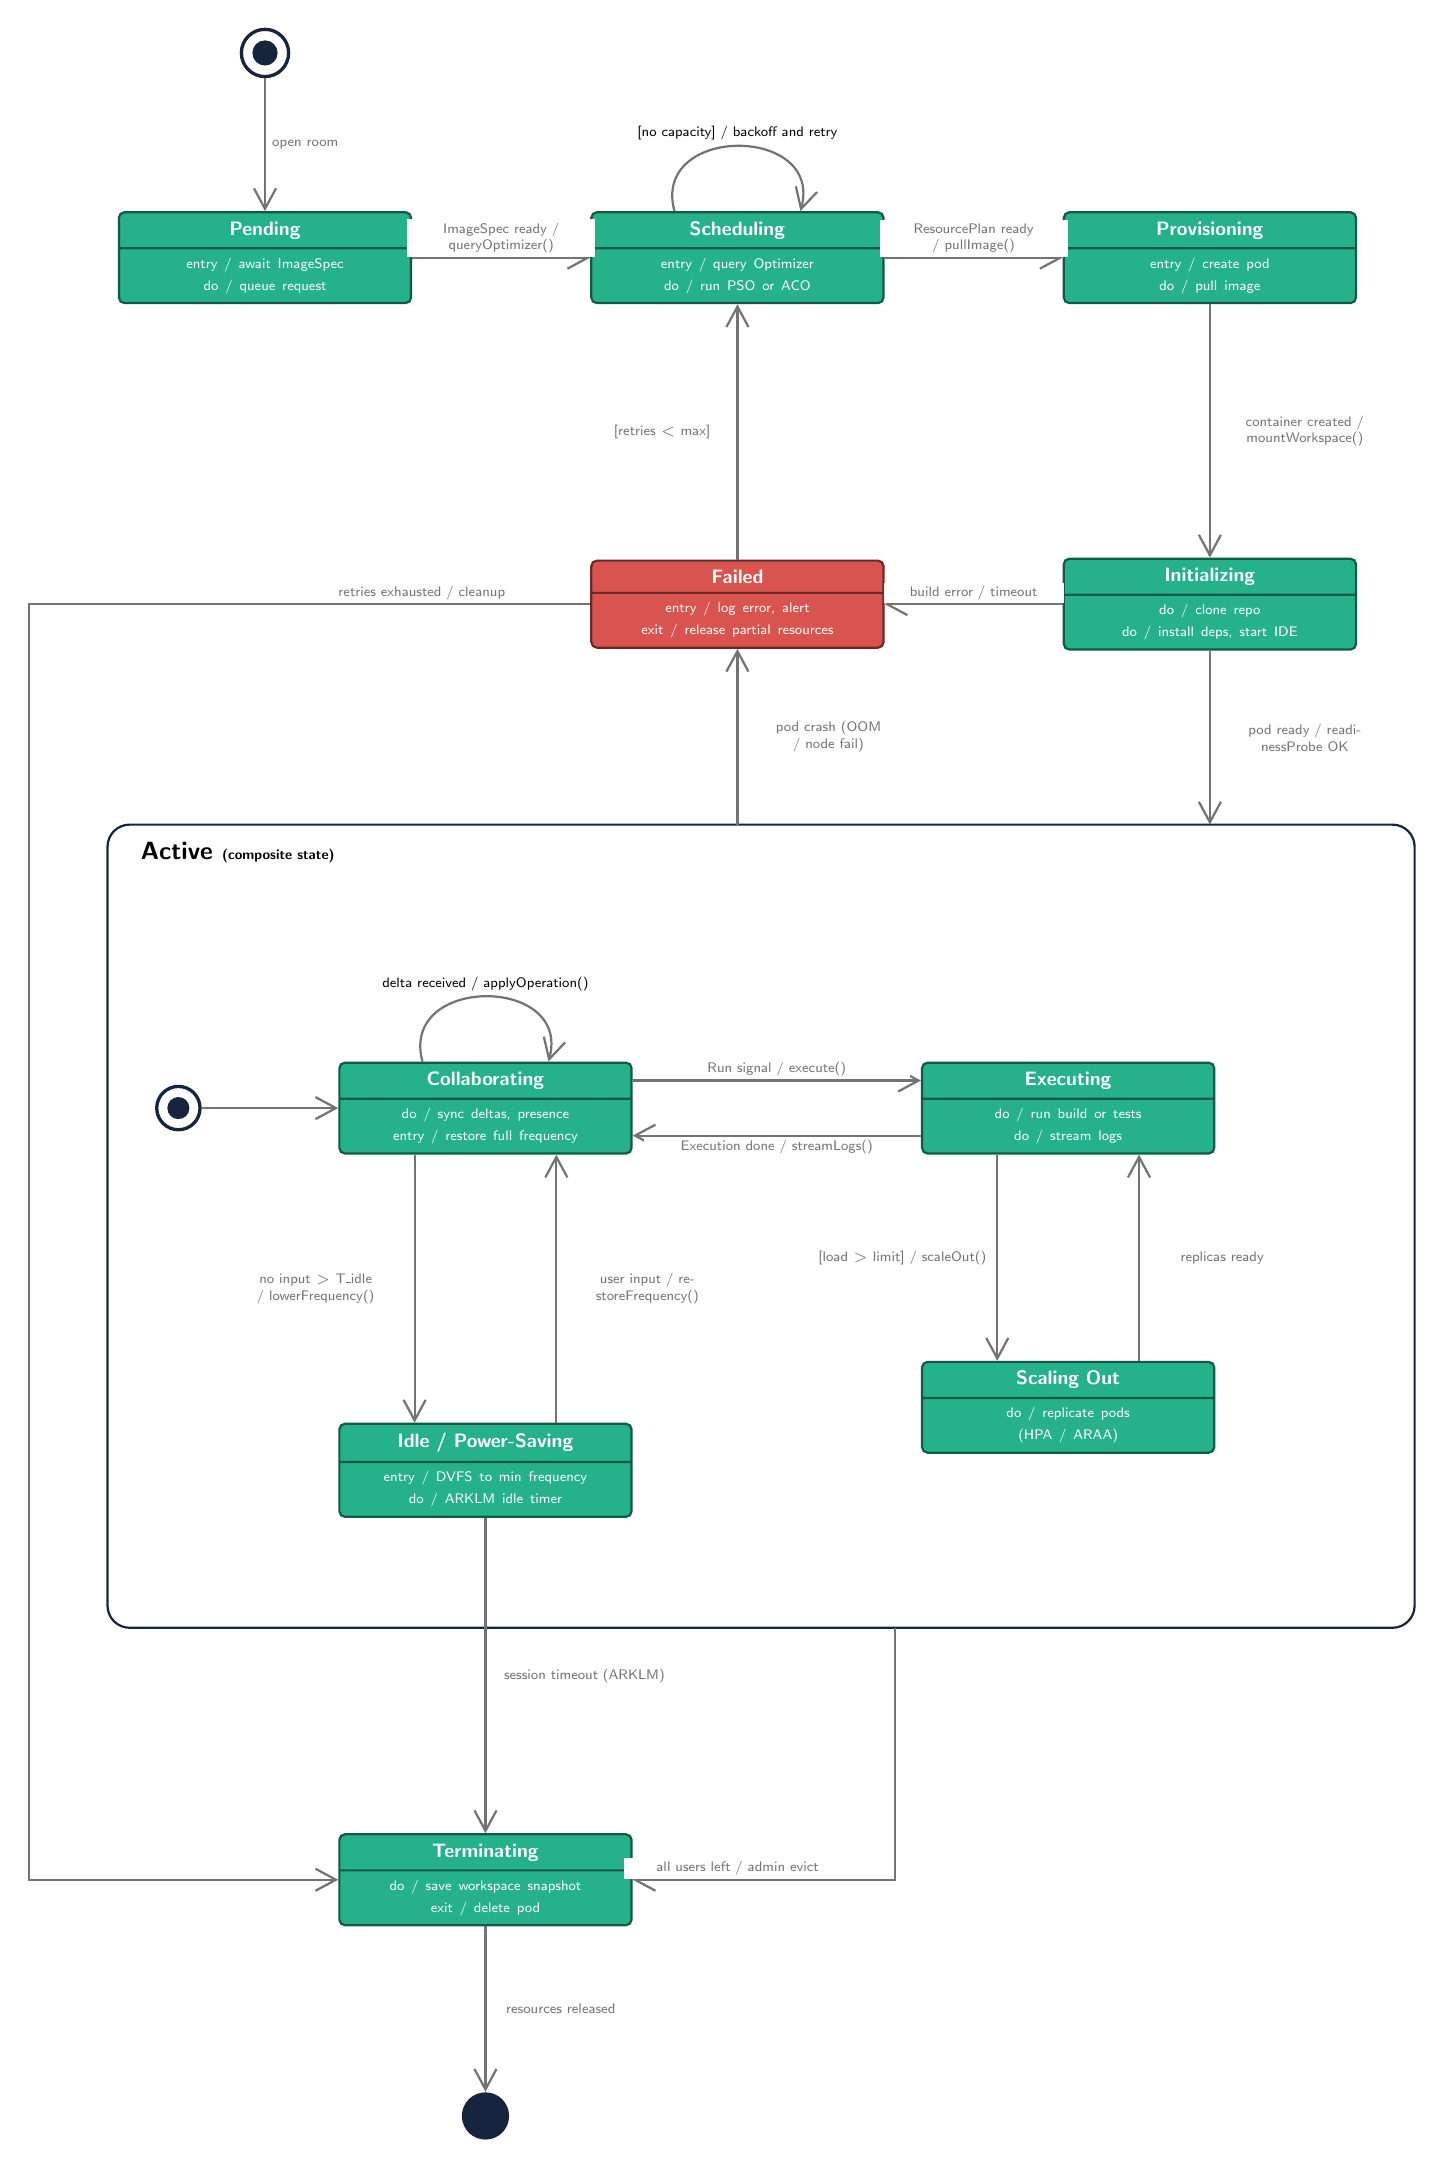
\begin{tikzpicture}[font=\scriptsize,
  st/.style={rectangle split, rectangle split parts=2, thick, rounded corners=2pt,
             text=white, text width=3.5cm, align=center, inner sep=3pt},
  tr/.style={-{Straight Barb[length=2.6mm,width=2.8mm]}, thick, black!55}]
% optional first argument = fill colour (default green, as in the reference)
\newcommand{\state}[5][grn]{\node[st,fill=#1,draw=#1!50!black] (#2) at (#3) {\textbf{#4}\nodepart{two}\tiny #5};}

% composite state boundary (drawn first)
\draw[thick, rounded corners=8pt, navy] (0,-7.2) rectangle (16.6,-17.4);
\node[anchor=north west,font=\small\bfseries] at (0.3,-7.3) {Active\ {\tiny(composite state)}};

% initial pseudo-state: ring with dot (reference style)
\node[circle,draw=navy,very thick,minimum size=0.6cm,inner sep=0] (i0) at (2,2.6) {};
\fill[navy] (i0) circle (0.16);
\state{pend}{2,0}{Pending}{entry / await ImageSpec\\do / queue request}
\state{sch}{8,0}{Scheduling}{entry / query Optimizer\\do / run PSO or ACO}
\state{prov}{14,0}{Provisioning}{entry / create pod\\do / pull image}
\state[redc]{fail}{8,-4.4}{Failed}{entry / log error, alert\\exit / release partial resources}
\state{init}{14,-4.4}{Initializing}{do / clone repo\\do / install deps, start IDE}

\node[circle,draw=navy,very thick,minimum size=0.55cm,inner sep=0] (i1) at (0.9,-10.8) {};
\fill[navy] (i1) circle (0.14);
\state{col}{4.8,-10.8}{Collaborating}{do / sync deltas, presence\\entry / restore full frequency}
\state{exe}{12.2,-10.8}{Executing}{do / run build or tests\\do / stream logs}
\state{scl}{12.2,-14.6}{Scaling Out}{do / replicate pods\\(HPA / ARAA)}
\state{idle}{4.8,-15.4}{Idle / Power-Saving}{entry / DVFS to min frequency\\do / ARKLM idle timer}

\state{term}{4.8,-20.6}{Terminating}{do / save workspace snapshot\\exit / delete pod}
% final state: solid dark disc (reference style)
\node[circle,fill=navy,minimum size=0.6cm,inner sep=0] (fin) at (4.8,-23.6) {};

% startup chain
\draw[tr] (i0) -- node[tl,right,xshift=1pt] {open room} (pend.north);
\draw[tr] (pend.east) -- node[tl,above,text width=2.3cm] {ImageSpec ready / queryOptimizer()} (sch.west);
\draw[tr] (sch.east) -- node[tl,above,text width=2.3cm] {ResourcePlan ready / pullImage()} (prov.west);
\draw[tr] ([xshift=-0.8cm]sch.north) .. controls +(-0.3,1.1) and +(0.3,1.1) .. ([xshift=0.8cm]sch.north);
\node[tl,above,text width=3.2cm] at ($(sch.north)+(0,0.85)$) {[no capacity] / backoff and retry};
\draw[tr] (prov.south) -- node[tl,right,text width=2.3cm] {container created / mountWorkspace()} (init.north);
\draw[tr] (init.west) -- node[tl,above,text width=2.2cm] {build error / timeout} (fail.east);
\draw[tr] (fail.north) -- node[tl,left,text width=1.8cm] {[retries \LT\ max]} (sch.south);
\draw[tr] (init.south) -- node[tl,right,text width=2.3cm] {pod ready / readinessProbe OK} (14,-7.2);
\draw[tr] (8,-7.2) -- node[tl,right,text width=2.2cm] {pod crash (OOM / node fail)} (fail.south);
\draw[tr] (fail.west) -- node[tl,above,pos=0.3,text width=2.4cm] {retries exhausted / cleanup} (-1.0,-4.4) -- (-1.0,-20.6) -- (term.west);

% active region
\draw[tr] (i1) -- (col.west);
\draw[tr] ([xshift=-0.8cm]col.north) .. controls +(-0.3,1.1) and +(0.3,1.1) .. ([xshift=0.8cm]col.north);
\node[tl,above,text width=3.2cm] at ($(col.north)+(0,0.85)$) {delta received / applyOperation()};
\draw[tr] ([yshift=3.5mm]col.east) -- node[tl,above,text width=3.3cm] {Run signal / execute()} ([yshift=3.5mm]exe.west);
\draw[tr] ([yshift=-3.5mm]exe.west) -- node[tl,below,text width=3.3cm] {Execution done / streamLogs()} ([yshift=-3.5mm]col.east);
\draw[tr] ([xshift=-9mm]exe.south) -- node[tl,left,text width=2.3cm] {[load \GT\ limit] / scaleOut()} ([xshift=-9mm]scl.north);
\draw[tr] ([xshift=9mm]scl.north) -- node[tl,right,text width=2.0cm] {replicas ready} ([xshift=9mm]exe.south);
\draw[tr] ([xshift=-9mm]col.south) -- node[tl,left,text width=2.4cm] {no input \GT\ T\_idle / lowerFrequency()} ([xshift=-9mm]idle.north);
\draw[tr] ([xshift=9mm]idle.north) -- node[tl,right,text width=2.2cm] {user input / restoreFrequency()} ([xshift=9mm]col.south);

% termination
\draw[tr] (idle.south) -- node[tl,right,text width=2.4cm] {session timeout (ARKLM)} (term.north);
\draw[tr] (10,-17.4) |- node[tl,above,pos=0.8,text width=2.8cm] {all users left / admin evict} (term.east);
\draw[tr] (term.south) -- node[tl,right,text width=1.8cm] {resources released} (fin.north);
\end{tikzpicture}}
\captionof{figure}{State Machine Diagram: Workspace Container Lifecycle}
\end{center}

% =====================================================================
% 5. ACTIVITY
% =====================================================================
\clearpage
\figtitle{5. Activity Diagram: Resource Allocation and Execution}
\begin{center}
\adjustbox{max width=\linewidth, max height=0.88\textheight}{%
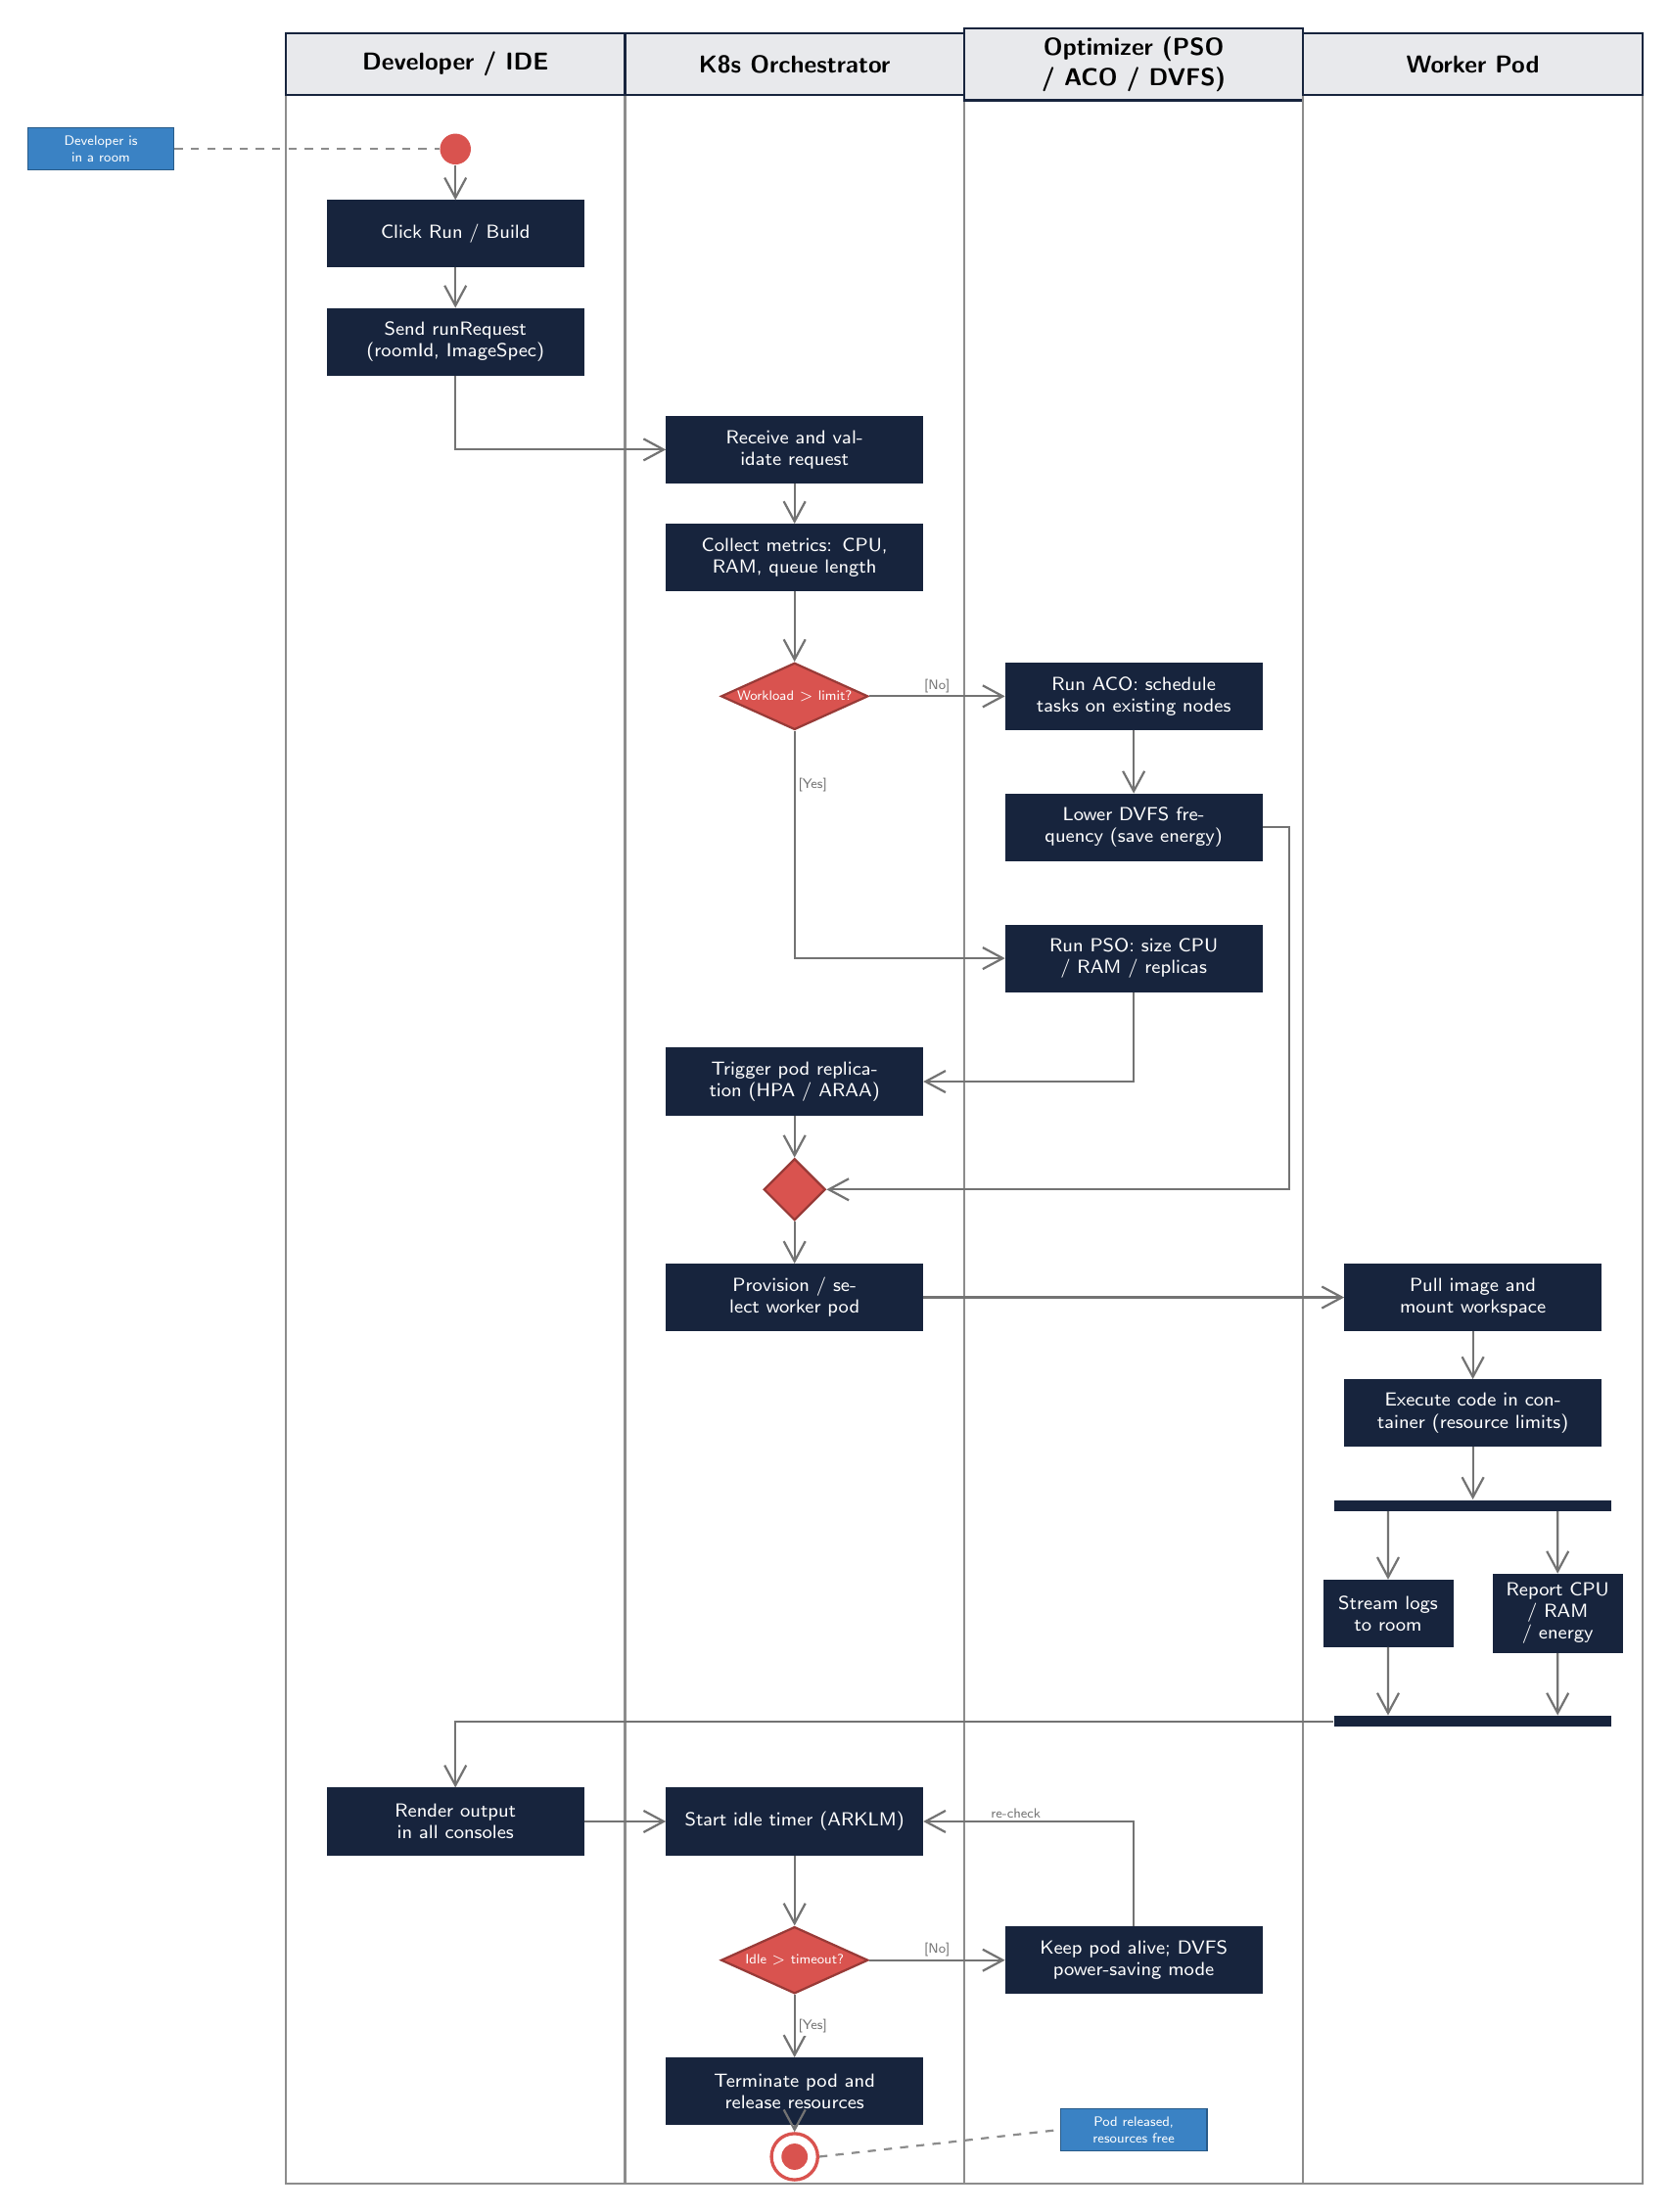
\begin{tikzpicture}[font=\scriptsize,
  act/.style={rectangle, draw=navy, thick, fill=navy, text=white, text width=3.1cm, align=center,
              minimum height=0.85cm, inner sep=3pt},
  dec/.style={diamond, aspect=2.2, draw=redc!70!black, thick, fill=redc, text=white, text width=1.6cm, align=center,
              inner sep=0pt, font=\tiny},
  fl/.style={-{Straight Barb[length=2.6mm,width=2.8mm]},thick,black!55},
  fb/.style={font=\tiny, fill=white, inner sep=1pt},
  bar/.style={rectangle, fill=navy, minimum height=0.14cm, inner sep=0},
  note/.style={rectangle, fill=blu, draw=blu!70!black, text=white, font=\tiny, align=center,
               inner sep=3pt, minimum width=1.9cm}]
% lanes
\def\xa{2.2}\def\xb{6.6}\def\xc{11.0}\def\xd{15.4}
\foreach \c/\t in {2.2/{Developer / IDE},6.6/{K8s Orchestrator},11.0/{Optimizer (PSO / ACO / DVFS)},15.4/{Worker Pod}}{
  \draw[thick,black!45] (\c-2.2,0) rectangle (\c+2.2,-27.9);
  \node[draw=navy,thick,fill=navy!10,minimum width=4.4cm,minimum height=0.8cm,font=\small\bfseries,text width=4.1cm,align=center] at (\c,-0.4) {\t};
}
\node[circle,fill=redc,minimum size=0.4cm,inner sep=0] (st) at (2.2,-1.5) {};
\node[act] (d1) at (2.2,-2.6) {Click Run / Build};
\node[act] (d2) at (2.2,-4.0) {Send runRequest\\(roomId, ImageSpec)};

\node[act] (o1) at (6.6,-5.4) {Receive and validate request};
\node[act] (o2) at (6.6,-6.8) {Collect metrics: CPU, RAM, queue length};
\node[dec] (dc) at (6.6,-8.6) {Workload \GT\ limit?};

\node[act] (aco) at (11.0,-8.6)  {Run ACO: schedule tasks on existing nodes};
\node[act] (dvl) at (11.0,-10.3) {Lower DVFS frequency (save energy)};
\node[act] (pso) at (11.0,-12.0) {Run PSO: size CPU / RAM / replicas};

\node[act] (o3) at (6.6,-13.6) {Trigger pod replication (HPA / ARAA)};
\node[diamond,draw=redc!70!black,thick,fill=redc,minimum width=0.8cm,minimum height=0.8cm,inner sep=0] (mg) at (6.6,-15.0) {};
\node[act] (o4) at (6.6,-16.4) {Provision / select worker pod};

\node[act] (p1) at (15.4,-16.4) {Pull image and mount workspace};
\node[act] (p2) at (15.4,-17.9) {Execute code in container (resource limits)};
\node[bar,minimum width=3.6cm] (fk) at (15.4,-19.1) {};
\node[act,text width=1.45cm] (p3) at (14.3,-20.5) {Stream logs to room};
\node[act,text width=1.45cm] (p4) at (16.5,-20.5) {Report CPU / RAM / energy};
\node[bar,minimum width=3.6cm] (jn) at (15.4,-21.9) {};

\node[act] (d3) at (2.2,-23.2) {Render output in all consoles};
\node[act] (o5) at (6.6,-23.2) {Start idle timer (ARKLM)};
\node[dec] (dc2) at (6.6,-25.0) {Idle \GT\ timeout?};
\node[act] (keep) at (11.0,-25.0) {Keep pod alive; DVFS power-saving mode};
\node[act] (o6) at (6.6,-26.7) {Terminate pod and release resources};
% final node: red ring with dot (reference style)
\node[circle,draw=redc,very thick,minimum size=0.6cm,inner sep=0] (fin) at (6.6,-27.55) {};
\fill[redc] (fin) circle (0.17);

% blue annotation notes, as in the reference
\node[note] (n1) at (-2.4,-1.5) {Developer is\\in a room};
\draw[dashed,thick,black!45] (n1.east) -- (st.west);
\node[note] (n2) at (11.0,-27.2) {Pod released,\\resources free};
\draw[dashed,thick,black!45] (fin.east) -- (n2.west);

\draw[fl] (st) -- (d1);
\draw[fl] (d1) -- (d2);
\draw[fl] (d2.south) |- (o1.west);
\draw[fl] (o1) -- (o2);
\draw[fl] (o2) -- (dc);
\draw[fl] (dc.east) -- node[fb,above] {[No]} (aco.west);
\draw[fl] (aco) -- (dvl);
\draw[fl] (dc.south) |- node[fb,pos=0.12,right] {[Yes]} (pso.west);
\draw[fl] (dvl.east) -- ++(0.35,0) |- (mg.east);
\draw[fl] (pso.south) |- (o3.east);
\draw[fl] (o3) -- (mg);
\draw[fl] (mg) -- (o4);
\draw[fl] (o4) -- (p1);
\draw[fl] (p1) -- (p2);
\draw[fl] (p2) -- (fk);
\draw[fl] ([xshift=-1.1cm]fk.south) -- (p3.north);
\draw[fl] ([xshift=1.1cm]fk.south) -- (p4.north);
\draw[fl] (p3.south) -- ([xshift=-1.1cm]jn.north);
\draw[fl] (p4.south) -- ([xshift=1.1cm]jn.north);
\draw[fl] (jn.west) -| (d3.north);
\draw[fl] (d3) -- (o5);
\draw[fl] (o5) -- (dc2);
\draw[fl] (dc2.east) -- node[fb,above] {[No]} (keep.west);
\draw[fl] (keep.north) |- node[fb,pos=0.78,above] {re-check} (o5.east);
\draw[fl] (dc2.south) -- node[fb,right] {[Yes]} (o6);
\draw[fl] (o6) -- (fin);
\end{tikzpicture}}
\captionof{figure}{Activity Diagram: Resource Allocation and Execution}
\end{center}

% =====================================================================
% 6. COMPONENT
% =====================================================================
\begin{landscape}
\figtitle{6. Component Diagram}
\begin{center}
\adjustbox{max width=\linewidth, max height=0.80\textheight}{%
\begin{tikzpicture}[font=\scriptsize,
  comp/.style={rectangle, draw=teal!70!black, thick, fill=white, minimum width=4.4cm, minimum height=2.0cm,
               align=center, inner sep=4pt},
  ext/.style={comp, dashed, draw=blu!80!black}]
\node[comp] (bro) at (0,6)   {{\tiny\gl{component}}\\\textbf{\small Browser Client}\\[2pt]{\tiny Monaco editor, WebSocket client}};
\node[comp] (gw)  at (9,6)   {{\tiny\gl{component}}\\\textbf{\small API Gateway}\\[2pt]{\tiny routing, JWT auth, WSS upgrade}};
\node[comp] (col) at (18,6)  {{\tiny\gl{component}}\\\textbf{\small Collab Engine}\\[2pt]{\tiny OT / CRDT sync, presence}};
\node[comp] (rep) at (9,1.8) {{\tiny\gl{component}}\\\textbf{\small Repo Service}\\[2pt]{\tiny clone, dependency scan}};
\node[ext]  (git) at (18,1.8){{\tiny\gl{external system}}\\\textbf{\small Git Host}\\[2pt]{\tiny GitHub / GitLab}};
\node[comp] (wrk) at (0,-2.4){{\tiny\gl{component}}\\\textbf{\small Worker Container}\\[2pt]{\tiny workspace runtime, DVFS-aware}};
\node[comp] (k8s) at (9,-2.4){{\tiny\gl{component}}\\\textbf{\small K8s Orchestrator}\\[2pt]{\tiny pod lifecycle, HPA / ARAA}};
\node[comp] (opt) at (18,-2.4){{\tiny\gl{component}}\\\textbf{\small Optimization Core}\\[2pt]{\tiny PSO, ACO, ARKLM}};
\foreach \n in {bro,gw,col,rep,wrk,k8s,opt} { \compicon{\n} }

% provider x y, requirer x y   (provider = ball, requirer = socket)
\iface{6.8}{6}{2.2}{6}{REST / WSS}{above=6pt}
\iface{15.8}{6}{11.2}{6}{OT Sync API}{above=6pt}
\iface{9}{2.8}{9}{5.0}{Git Ingestion}{right=7pt}
\iface{9}{-1.4}{9}{0.8}{ImageSpec Delivery}{right=7pt}
\iface{15.8}{-2.4}{11.2}{-2.4}{Schedule Engine}{above=6pt}
\iface{2.2}{-2.4}{6.8}{-2.4}{CRI Exec / Logs}{above=6pt}
\iface{0}{-1.4}{0}{5.0}{Terminal Stream}{right=7pt}
\iface{15.8}{1.8}{11.2}{1.8}{Git Clone API}{above=6pt}
\end{tikzpicture}}
\captionof{figure}{Component Diagram (ball = provided interface, socket = required interface)}
\end{center}
\end{landscape}

% =====================================================================
% 7. DEPLOYMENT
% =====================================================================
\begin{landscape}
\figtitle{7. Deployment Diagram}
\begin{center}
\adjustbox{max width=\linewidth, max height=0.80\textheight}{%
\begin{tikzpicture}[font=\scriptsize,
  art/.style={rectangle, draw=teal!70!black, thick, fill=white, align=center, text width=3.4cm, minimum height=1.1cm, inner sep=3pt},
  conn/.style={thick,black!60}]
% 3-D node: name, cx, cy, width, height, title
\newcommand{\dnode}[6]{%
  \node[draw=navy!80,thick,fill=teal!8,minimum width=#4 cm,minimum height=#5 cm,inner sep=0] (#1) at (#2,#3) {};
  \draw[thick,draw=navy!80,fill=teal!8] (#1.north west) -- ++(0.35,0.3) -- ($(#1.north east)+(0.35,0.3)$) -- (#1.north east) -- cycle;
  \draw[thick,draw=navy!80,fill=teal!8] (#1.north east) -- ++(0.35,0.3) -- ($(#1.south east)+(0.35,0.3)$) -- (#1.south east) -- cycle;
  \node[anchor=north,align=center,font=\scriptsize\bfseries,text width={#4 cm-0.4cm}] at ($(#1.north)+(0,-0.15)$) {#6};
  \draw[thick,navy!80] ($(#1.north west)+(0,-1.15)$) -- ($(#1.north east)+(0,-1.15)$);}
% artifact with component icon
\newcommand{\artifact}[5][3.4cm]{%
  \node[art,text width=#1] (#2) at (#3,#4) {{\tiny\gl{artifact}}\\\textbf{#5}};
  \compicon{#2}}

% Kubernetes cluster boundary
\draw[thick,dashed] (5.2,-8.0) rectangle (17.3,8.7);
\node[anchor=north west,font=\small\bfseries,fill=white,inner sep=2pt] at (5.4,8.65) {\gl{cluster} Kubernetes Cluster};

\dnode{cli}{-1.2}{0}{5.0}{4.4}{\gl{device}\\Developer Client PC}
\node[font=\tiny,align=center] at (-1.2,0.55) {OS: Linux / macOS / Windows};
\artifact{browser}{-1.2}{-1.0}{Web Browser\\{\tiny Monaco Editor, WASM}}

\dnode{mas}{11.2}{4.9}{10.0}{5.5}{\gl{execution environment}\\K8s Master Node}
\node[font=\tiny] at (11.2,6.2) {Control plane (Ubuntu 24.04 LTS)};
\artifact{gw}{8.8}{4.9}{API Gateway Pod}
\artifact{ce}{13.6}{4.9}{Collab Engine Pod}
\artifact{rs}{8.8}{3.4}{Repo Service Pod}
\artifact{oe}{13.6}{3.4}{PSO / ACO Engine}

\dnode{wrk}{11.2}{-4.6}{10.0}{5.0}{\gl{execution environment}\\K8s Worker Node (AMD / Intel, DVFS)}
\node[font=\tiny] at (11.2,-3.45) {Hardware layer: cpufreq / acpi-cpufreq governor};
\artifact[2.7cm]{p1}{8.0}{-5.3}{Workspace Pod 1\\{\tiny Docker / Node}}
\artifact[2.7cm]{p2}{11.2}{-5.3}{Workspace Pod 2\\{\tiny Docker / Python}}
\artifact[2.7cm]{kl}{14.4}{-5.3}{Kubelet + DVFS agent}

\dnode{sto}{23.2}{-4.6}{6.0}{4.0}{\gl{device}\\Persistent Cluster Storage}
\node[font=\tiny] at (23.2,-4.05) {Storage engine: Ceph RBD / NFS};
\artifact{vol}{23.2}{-5.4}{Project Volume Shares\\{\tiny Git cache}}

% communication paths
\draw[conn] (cli.east) -- node[tl,above,sloped,pos=0.5] {HTTPS / WSS (443)} (mas.west);
\draw[conn] (cli.south east) -- node[tl,below,sloped,pos=0.45] {Terminal stream (WSS)} (wrk.west);
\draw[conn] (mas.south) -- node[tl,right,xshift=2pt] {Kubelet gRPC (10250)} (wrk.north);
\draw[conn] (wrk.east) -- node[tl,above,text width=2.4cm] {CSI iSCSI / NFS mount} (sto.west);
\end{tikzpicture}}
\captionof{figure}{Deployment Diagram}
\end{center}
\end{landscape}

% =====================================================================
% 8. OBJECT
% =====================================================================
\clearpage
\figtitle{8. Object Diagram (Runtime Instance Snapshot)}
\begin{center}
\adjustbox{max width=\linewidth, max height=0.86\textheight}{%
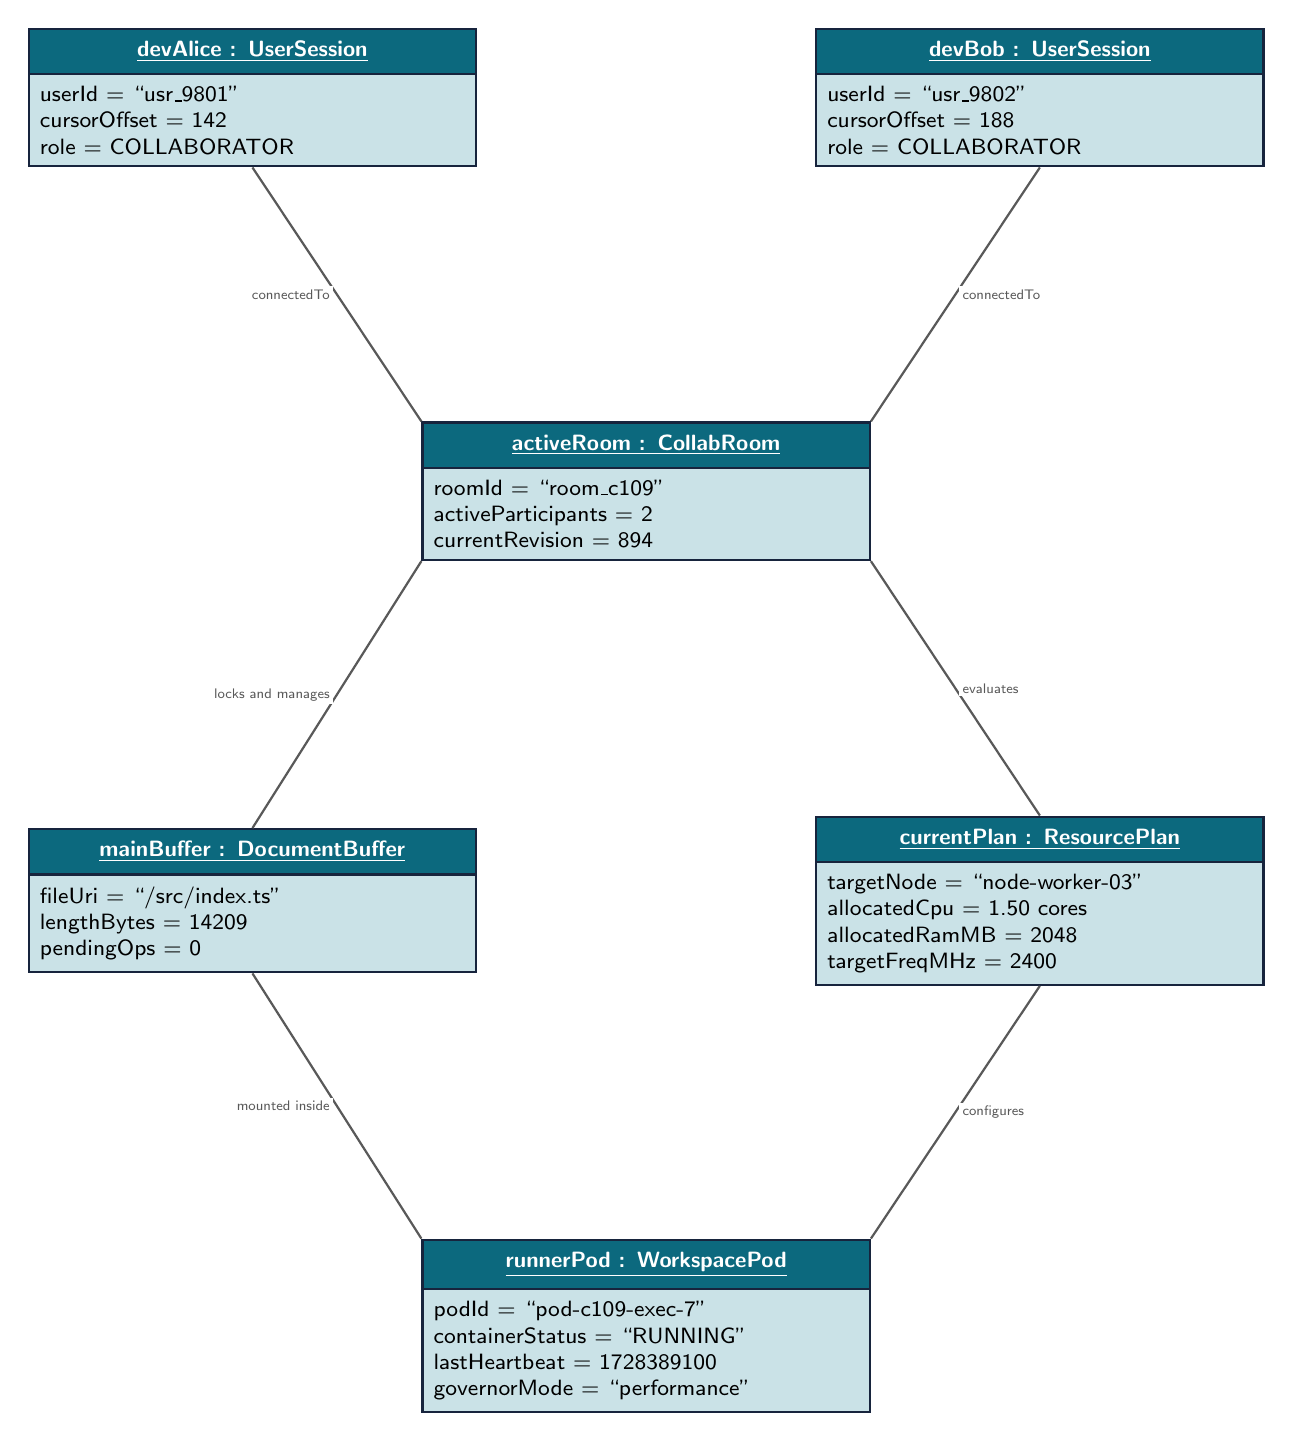
\begin{tikzpicture}[font=\footnotesize,
  obj/.style={rectangle split, rectangle split parts=2, draw=navy, thick,
              rectangle split part fill={teal!85!black,teal!22},
              text width=5.4cm, align=left, inner sep=4pt}]
\newcommand{\inst}[4]{\node[obj] (#1) at (#2) {{\centering\color{white}\underline{\textbf{#3}}\par}\nodepart{two}#4};}

\inst{alice}{0,0}{devAlice : UserSession}{userId = ``usr\_9801''\\cursorOffset = 142\\role = COLLABORATOR}
\inst{bob}{10,0}{devBob : UserSession}{userId = ``usr\_9802''\\cursorOffset = 188\\role = COLLABORATOR}
\inst{room}{5,-5.0}{activeRoom : CollabRoom}{roomId = ``room\_c109''\\activeParticipants = 2\\currentRevision = 894}
\inst{doc}{0,-10.2}{mainBuffer : DocumentBuffer}{fileUri = ``/src/index.ts''\\lengthBytes = 14209\\pendingOps = 0}
\inst{plan}{10,-10.2}{currentPlan : ResourcePlan}{targetNode = ``node-worker-03''\\allocatedCpu = 1.50 cores\\allocatedRamMB = 2048\\targetFreqMHz = 2400}
\inst{pod}{5,-15.6}{runnerPod : WorkspacePod}{podId = ``pod-c109-exec-7''\\containerStatus = ``RUNNING''\\lastHeartbeat = 1728389100\\governorMode = ``performance''}

\draw[thick,black!65] (alice.south) -- (room.north west) node[lbl,pos=0.5,left=1pt] {connectedTo};
\draw[thick,black!65] (bob.south) -- (room.north east) node[lbl,pos=0.5,right=1pt] {connectedTo};
\draw[thick,black!65] (room.south west) -- (doc.north) node[lbl,pos=0.5,left=1pt] {locks and manages};
\draw[thick,black!65] (room.south east) -- (plan.north) node[lbl,pos=0.5,right=1pt] {evaluates};
\draw[thick,black!65] (plan.south) -- (pod.north east) node[lbl,pos=0.5,right=1pt] {configures};
\draw[thick,black!65] (doc.south) -- (pod.north west) node[lbl,pos=0.5,left=1pt] {mounted inside};
\end{tikzpicture}}
\captionof{figure}{Object Diagram (Runtime Instance Snapshot)}
\end{center}

% =====================================================================
% 9. COLLABORATION (COMMUNICATION)  -- reference style:
%    actor / boundary / control / entity icons, numbered messages
% =====================================================================
\begin{landscape}
\figtitle{9. Collaboration (Communication) Diagram}
\begin{center}
\adjustbox{max width=\linewidth, max height=0.80\textheight}{%
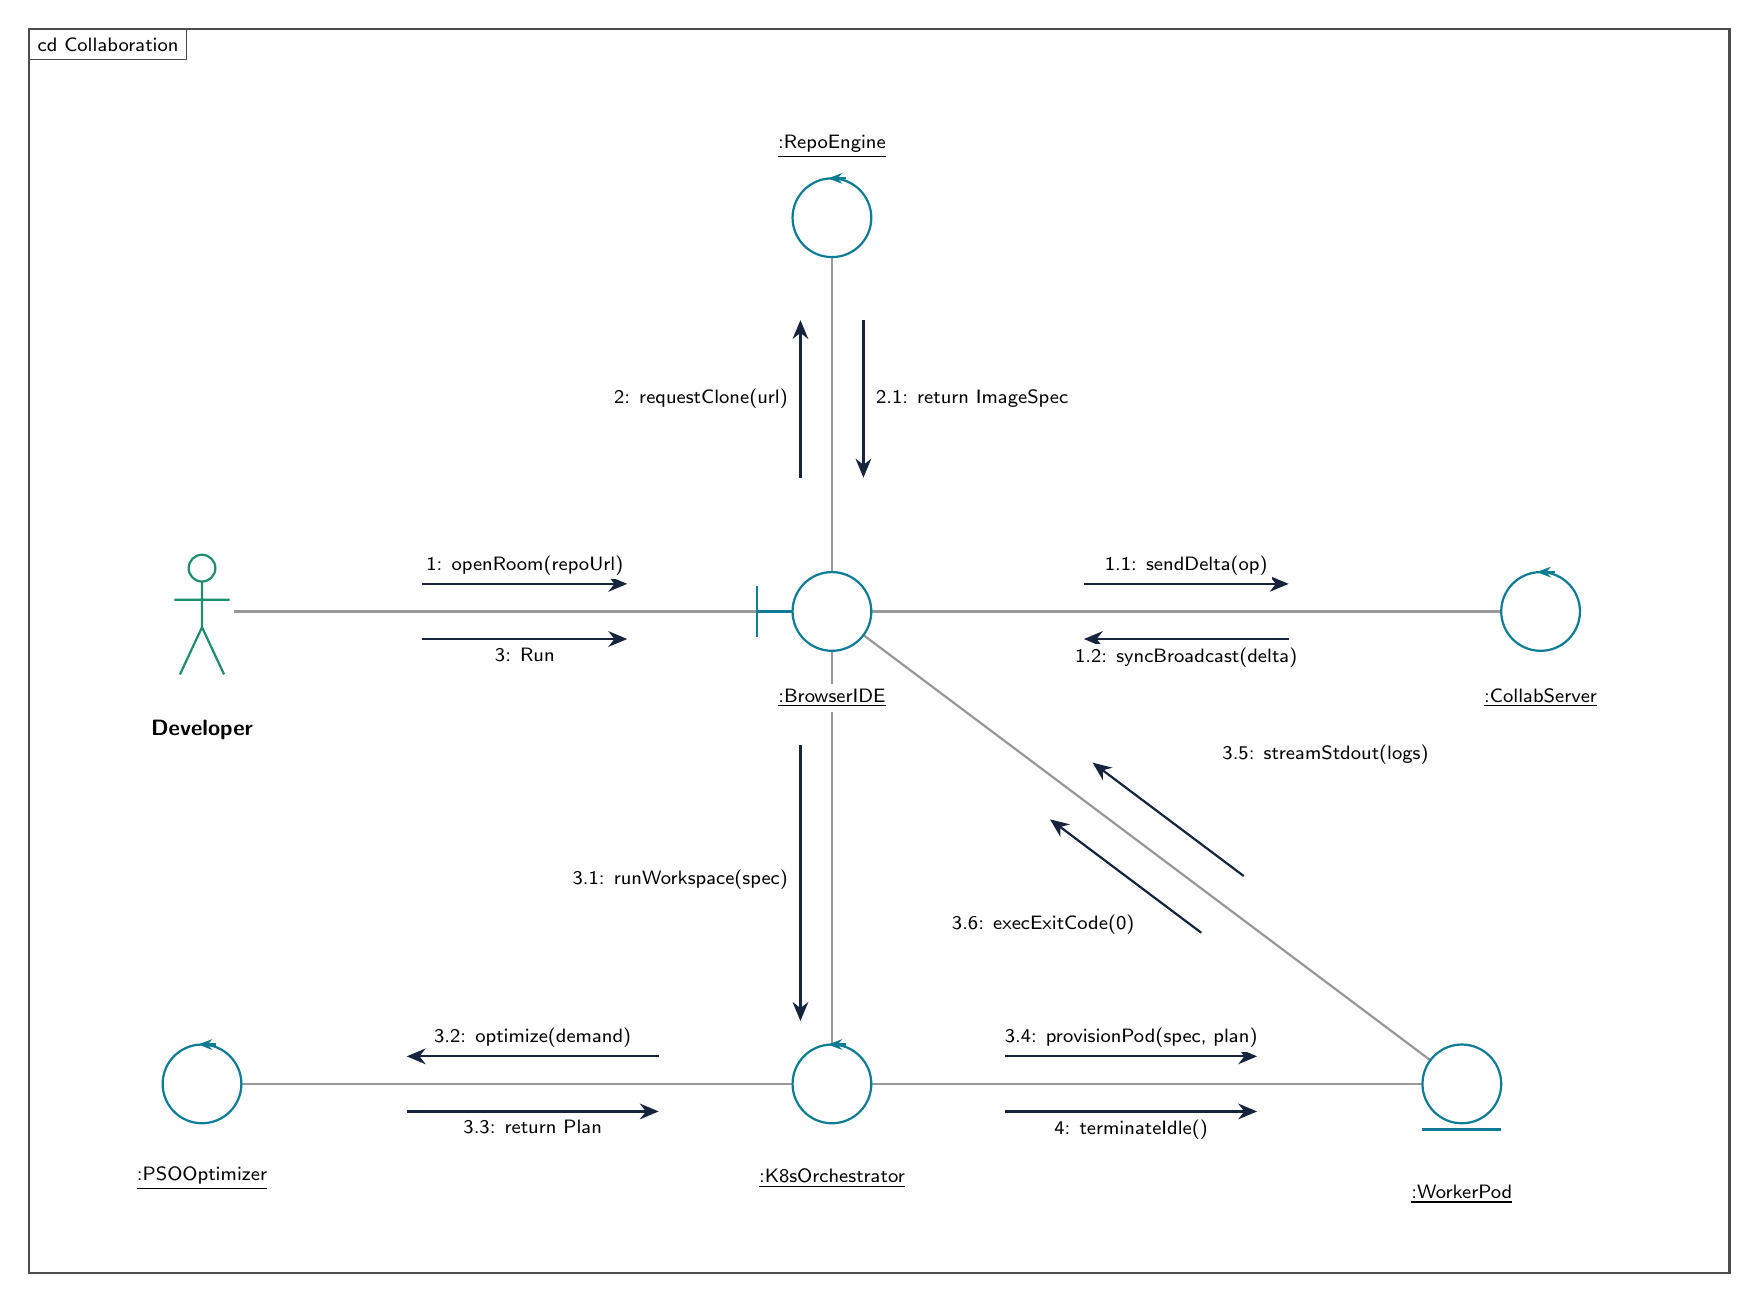
\begin{tikzpicture}[font=\scriptsize,
  lk/.style={black!40,thick},
  ma/.style={-{Stealth[length=2.4mm,width=2mm]},thick,navy},
  mt/.style={font=\scriptsize, inner sep=1.5pt, fill=white}]
% icons: label, centre, label-position
\newcommand{\bnd}[3]{%
  \draw[thick,teal] ($(#2)+(-0.5,0)$) -- ++(-0.45,0);
  \draw[thick,teal] ($(#2)+(-0.95,0.32)$) -- ++(0,-0.64);
  \draw[thick,teal,fill=white] (#2) circle (0.5);
  \node[mt] at (#3) {\underline{#1}};}
\newcommand{\ctl}[3]{%
  \draw[thick,teal,fill=white] (#2) circle (0.5);
  \draw[thick,teal,-{Stealth[length=1.8mm]}] ($(#2)+(0.18,0.5)$) -- ($(#2)+(-0.05,0.5)$);
  \node[mt] at (#3) {\underline{#1}};}
\newcommand{\ent}[3]{%
  \draw[thick,teal,fill=white] (#2) circle (0.5);
  \draw[thick,teal] ($(#2)+(-0.5,-0.58)$) -- ($(#2)+(0.5,-0.58)$);
  \node[mt] at (#3) {\underline{#1}};}

% frame
\draw[black!70,thick] (-2.2,-5.4) rectangle (19.4,10.4);
\node[anchor=north west,draw=black!70,fill=white,font=\scriptsize,inner sep=3pt] at (-2.2,10.4) {cd Collaboration};

% links (drawn first, icons sit on top)
\draw[lk] (0.4,3) -- (8,3);
\draw[lk] (8,3) -- (17,3);
\draw[lk] (8,3) -- (8,8);
\draw[lk] (8,3) -- (8,-3);
\draw[lk] (8,-3) -- (0,-3);
\draw[lk] (8,-3) -- (16,-3);
\draw[lk] (16,-3) -- (8,3);

% objects
\begin{scope}[draw=grn!80!black]
  \actor{dev}{0}{3}{Developer}
\end{scope}
\bnd{:BrowserIDE}{8,3}{8,1.9}
\ctl{:CollabServer}{17,3}{17,1.9}
\ctl{:RepoEngine}{8,8}{8,8.9}
\ctl{:K8sOrchestrator}{8,-3}{8,-4.2}
\ctl{:PSOOptimizer}{0,-3}{0,-4.2}
\ent{:WorkerPod}{16,-3}{16,-4.4}

% Developer <-> IDE
\draw[ma] (2.8,3.35) -- (5.4,3.35);
\node[mt,anchor=south] at (4.1,3.4) {1: openRoom(repoUrl)};
\draw[ma] (2.8,2.65) -- (5.4,2.65);
\node[mt,anchor=north] at (4.1,2.6) {3: Run};

% IDE <-> Collab
\draw[ma] (11.2,3.35) -- (13.8,3.35);
\node[mt,anchor=south] at (12.5,3.4) {1.1: sendDelta(op)};
\draw[ma] (13.8,2.65) -- (11.2,2.65);
\node[mt,anchor=north] at (12.5,2.6) {1.2: syncBroadcast(delta)};

% IDE <-> Repo
\draw[ma] (7.6,4.7) -- (7.6,6.7);
\node[mt,anchor=east] at (7.5,5.7) {2: requestClone(url)};
\draw[ma] (8.4,6.7) -- (8.4,4.7);
\node[mt,anchor=west] at (8.5,5.7) {2.1: return ImageSpec};

% IDE -> K8s
\draw[ma] (7.6,1.3) -- (7.6,-2.2);
\node[mt,anchor=east] at (7.5,-0.4) {3.1: runWorkspace(spec)};

% K8s <-> Optimizer
\draw[ma] (5.8,-2.65) -- (2.6,-2.65);
\node[mt,anchor=south] at (4.2,-2.6) {3.2: optimize(demand)};
\draw[ma] (2.6,-3.35) -- (5.8,-3.35);
\node[mt,anchor=north] at (4.2,-3.4) {3.3: return Plan};

% K8s -> Pod
\draw[ma] (10.2,-2.65) -- (13.4,-2.65);
\node[mt,anchor=south] at (11.8,-2.6) {3.4: provisionPod(spec, plan)};
\draw[ma] (10.2,-3.35) -- (13.4,-3.35);
\node[mt,anchor=north] at (11.8,-3.4) {4: terminateIdle()};

% Pod -> IDE (diagonal link)
\draw[ma] (13.23,-0.36) -- (11.31,1.08);
\node[mt,anchor=south west] at (12.9,1.0) {3.5: streamStdout(logs)};
\draw[ma] (12.69,-1.08) -- (10.77,0.36);
\node[mt,anchor=north east] at (11.9,-0.8) {3.6: execExitCode(0)};
\end{tikzpicture}}
\captionof{figure}{Collaboration (Communication) Diagram}
\end{center}
\end{landscape}

% =====================================================================
% 10. PACKAGE DIAGRAM  (new, matches the reference)
% =====================================================================
\begin{landscape}
\figtitle{10. Package Diagram}
\begin{center}
\adjustbox{max width=\linewidth, max height=0.80\textheight}{%
\begin{tikzpicture}[font=\scriptsize,
  pkgbody/.style={rectangle,draw=teal!70!black,thick,fill=white,text width=5.2cm,minimum height=2.9cm,
                  align=left,inner sep=6pt},
  pkgtab/.style={rectangle,draw=teal!70!black,thick,fill=white,font=\scriptsize\bfseries,
                 inner sep=3pt,anchor=south west}]
\newcommand{\pkg}[4]{\node[pkgbody] (#1) at (#2) {#4}; \node[pkgtab] at (#1.north west) {#3};}

\pkg{cl}{9,0}{Client}{+ BrowserIDE\\+ MonacoEditor\\+ WebSocketClient}
\pkg{co}{0,-6}{Collaboration}{+ UserSession\\+ CollabRoom\\+ DocumentBuffer\\+ TextOp\\+ OTEngine}
\pkg{pr}{9,-6}{Provisioning}{+ RepositoryAnalyzer\\+ ImageSpec\\+ WorkspacePod\\+ K8sPodManager\\+ HealthState}
\pkg{op}{18,-6}{Optimization}{+ IClusterOptimizer\\+ PSOContainerSizer\\+ ACOScheduler\\+ ARKLMReclaimer\\+ DVFSGovernor}
\pkg{inf}{9,-12}{Infrastructure}{+ Kubernetes API\\+ Git Host\\+ Cluster Storage}

\draw[dep] (cl.west) -| (co.north) node[lbl,pos=0.25,above] {\gl{uses}};
\draw[dep] (cl.south) -- (pr.north) node[lbl,pos=0.5,right] {\gl{uses}};
\draw[dep] (pr.east) -- (op.west) node[lbl,pos=0.5,above] {\gl{uses}};
\draw[dep] (pr.south) -- (inf.north) node[lbl,pos=0.5,right] {\gl{uses}};
\draw[dep] (op.south) |- (inf.east) node[lbl,pos=0.75,above] {\gl{uses}};
\end{tikzpicture}}
\captionof{figure}{Package Diagram: dependencies between the platform's packages}
\end{center}
\end{landscape}

% =====================================================================
% 11. COMPOSITE STRUCTURE DIAGRAM  (new, matches the reference)
% =====================================================================
\begin{landscape}
\figtitle{11. Composite Structure Diagram}
\begin{center}
\adjustbox{max width=\linewidth, max height=0.80\textheight}{%
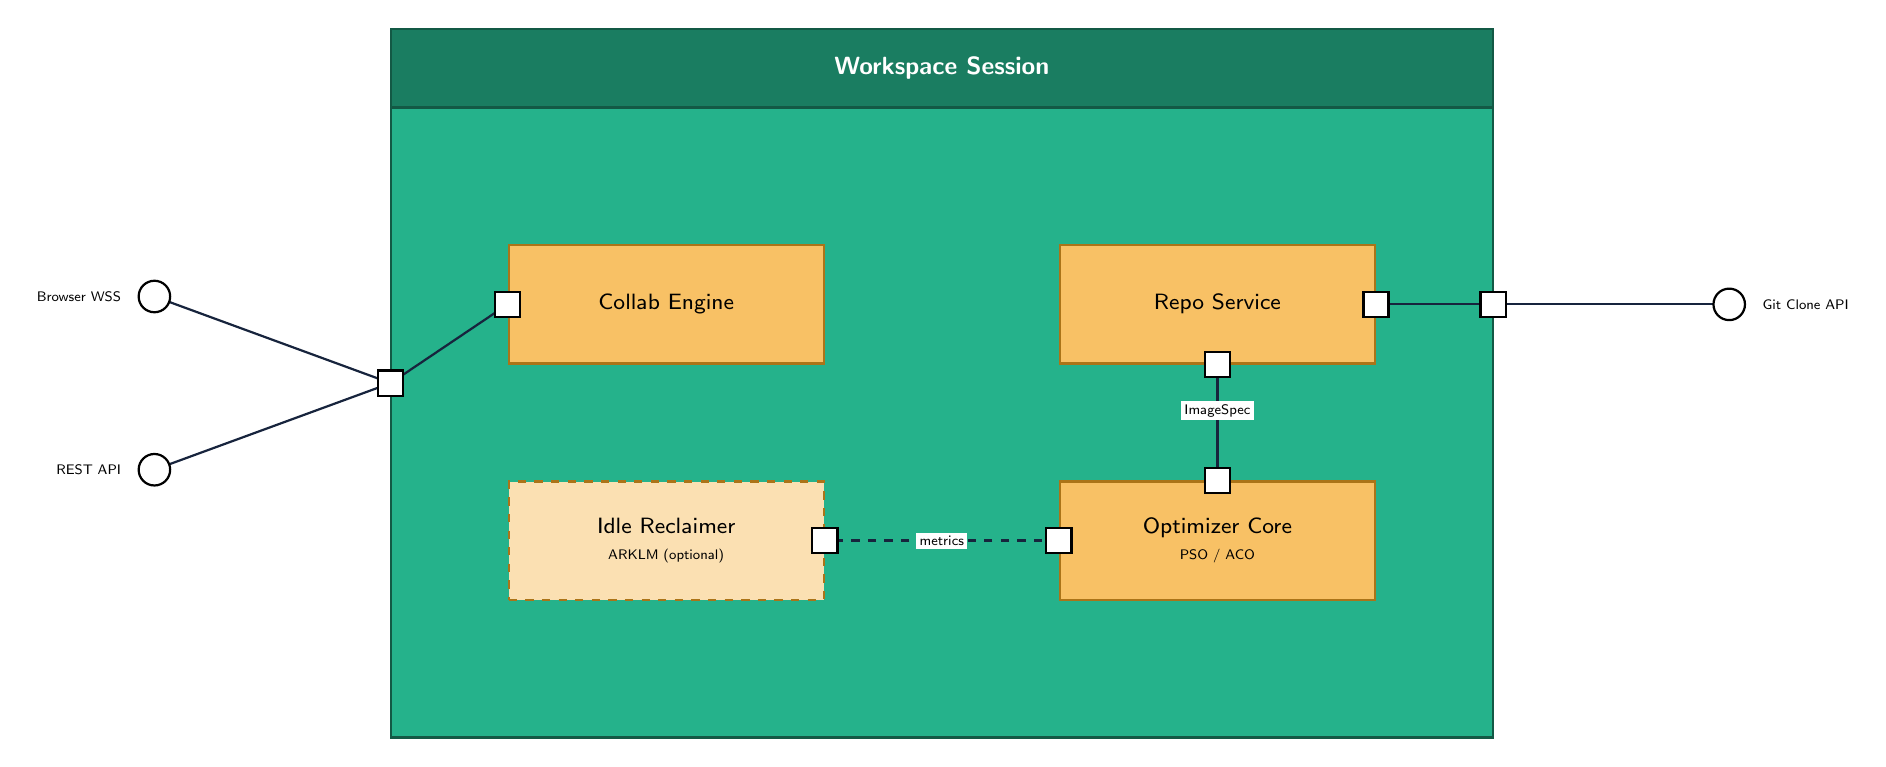
\begin{tikzpicture}[font=\scriptsize,
  part/.style={rectangle,draw=ora!70!black,thick,fill=ora!70,minimum width=4cm,minimum height=1.5cm,
               align=center,font=\footnotesize},
  port/.style={rectangle,draw=black,thick,fill=white,minimum size=0.32cm,inner sep=0},
  wire/.style={thick,navy}]

% enclosing class (green, with header band)
\draw[thick,draw=grn!50!black,fill=grn] (0,0) rectangle (14,-9);
\draw[thick,draw=grn!50!black,fill=grn!70!black] (0,0) rectangle (14,-1);
\node[font=\small\bfseries,text=white] at (7,-0.5) {Workspace Session};

% parts
\node[part] (pc) at (3.5,-3.5) {Collab Engine};
\node[part] (pr) at (10.5,-3.5) {Repo Service};
\node[part] (po) at (10.5,-6.5) {Optimizer Core\\{\tiny PSO / ACO}};
\node[part,dashed,fill=ora!35] (pi) at (3.5,-6.5) {Idle Reclaimer\\{\tiny ARKLM (optional)}};

% wires (drawn before ports)
\draw[wire] (0,-4.5) -- (pc.west);
\draw[wire] (pr.east) -- (14,-3.5);
\draw[wire] (pr.south) -- (po.north);
\draw[wire,dashed] (po.west) -- (pi.east);
\draw[wire] (-3,-3.4) -- (0,-4.5);
\draw[wire] (-3,-5.6) -- (0,-4.5);
\draw[wire] (14,-3.5) -- (17,-3.5);

% required/provided interface circles outside the class
\draw[thick,fill=white] (-3,-3.4) circle (0.2);
\draw[thick,fill=white] (-3,-5.6) circle (0.2);
\draw[thick,fill=white] (17,-3.5) circle (0.2);
\node[font=\tiny,anchor=east] at (-3.3,-3.4) {Browser WSS};
\node[font=\tiny,anchor=east] at (-3.3,-5.6) {REST API};
\node[font=\tiny,anchor=west] at (17.3,-3.5) {Git Clone API};
\node[lbl] at (10.5,-4.85) {ImageSpec};
\node[lbl] at (7.0,-6.5) {metrics};

% ports
\node[port] at (0,-4.5) {};
\node[port] at (pc.west) {};
\node[port] at (pr.east) {};
\node[port] at (14,-3.5) {};
\node[port] at (pr.south) {};
\node[port] at (po.north) {};
\node[port] at (po.west) {};
\node[port] at (pi.east) {};
\end{tikzpicture}}
\captionof{figure}{Composite Structure Diagram: internal structure of a workspace session}
\end{center}
\end{landscape}
\end{document}